\documentclass[a4paper,12pt]{article}
\usepackage[T1]{fontenc}
\usepackage[utf8]{inputenc}
\usepackage{polski}
\usepackage{color}
\usepackage{graphicx}
\usepackage{amsmath}
\usepackage{amssymb}
\usepackage{hyperref}
\usepackage{float}
\usepackage{listings}

\lstset{
  basicstyle=\ttfamily,
  columns=flexible,
  keepspaces=true,
  literate={ą}{{\k{a}}}1
           {ć}{{\'{c}}}1
           {ę}{{\k{e}}}1
           {ł}{{\l{}}}1
           {ń}{{\'{n}}}1
           {ó}{{\'{o}}}1
           {ś}{{\'{s}}}1
           {ź}{{\'{z}}}1
           {ż}{{\dot{z}}}1
           {Ą}{{\k{A}}}1
           {Ć}{{\'{C}}}1
           {Ę}{{\k{E}}}1
           {Ł}{{\L{}}}1
           {Ń}{{\'{N}}}1
           {Ó}{{\'{O}}}1
           {Ś}{{\'{S}}}1
           {Ź}{{\'{Z}}}1
           {Ż}{{\dot{Z}}}1
}

\title{Sprawozdanie z laboratorium Hurtownie Danych}
\author{Mikołaj Kubś, 272662}
\date{\today}

\begin{document}

\maketitle

\section{Zadanie 1}
Analiza konceptualnego modelu danych "Usługi", który jest niekompletny,
ale klasy i relacje między nimi reprezentują rozpatrywany wycinek rzeczywistości. 

\begin{figure}[H]
\centering
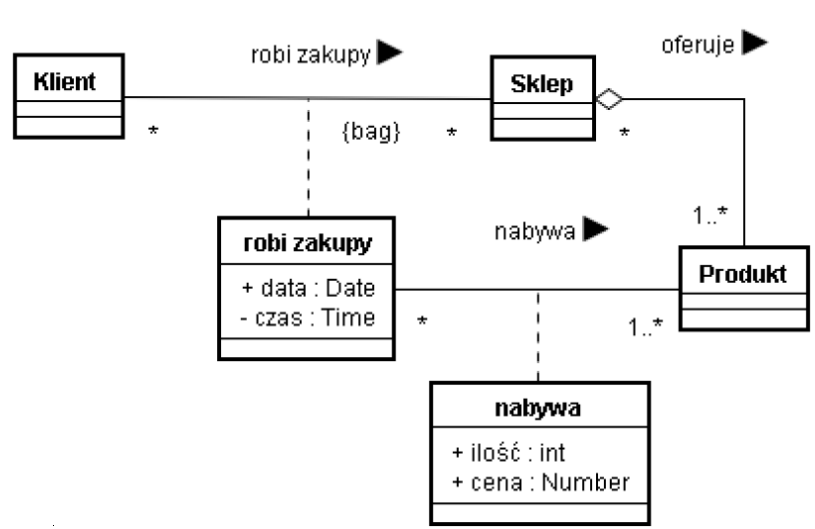
\includegraphics[width=0.8\textwidth]{images/old.png}
\caption{Konceptualny model danych "Usługi"}
\label{fig:uslugi}
\end{figure}

Reguły i ograniczenia dziedzinowe:
\begin{itemize}
    \item Reg/01 - Klient może wielokrotnie robić zakupy w tym samym sklepie
    \item Reg/02 - W sklepie może robić zakupy dowolny klient
    \item Reg/03 - Każdy zakup realizowany jest przez klienta w sklepie w określonym dniu i godzinie
    \item Reg/04 - Sklep musi oferować co najmniej jeden produkt
    \item Reg/05 - \ldots
\end{itemize}

\subsection{Weryfikacja i poprawa modelu danych}

Ponieważ reguły są niekompletne i nie w pełni poprawne, zdecydowałem się wprowadzić szereg zmian. 

Uznałem, że reguła "Reg/04 - Sklep musi oferować co najmniej jeden produkt" wprowadza niepotrzebną komplikację. Na przykład, według tej zasady, gdy sklep sprzedałby cały swój inwentarz, nie mógłby dalej istnieć w bazie danych.

Brakuje aktualnie informacji, jaka jest liczba dostępnego produktu w danym sklepie. Można wyciągnąć tę daną do nowej tabeli asocjacyjnej, do której można by dodatkowo dodać cenę produktu dla konkretnego sklepu, co zwiększa elastyczność na przyszłość i jest szeroko stosowaną praktyką w rzeczywistych sklepach. Tak więc sklep może oferować wiele produktów, każdy z własną cenę i ilością. 
Ponieważ tabela asocjacyjna "oferuje" ma cenę, można by usunąć cenę z tabeli asocjacyjnej "nabywa". Uznałem jednak, że ją zostawię, ponieważ cena oferty może się zmienić po zakupie produktu przez klienta. 
Sklepy mają często informację, że coś sprzedają, nawet jeśli nie ma tego chwilowo w magazynie, tak więc ustaliłem, że ilość oferowanego produktu to co najmniej 0, a nie koniecznie więcej niż zero, co wymuszałoby usunięcie oferty w przypadku braków w magazynie.

Można dodać parę atrybutów do encji. Do klienta dodam imię i nazwisko, a do produktu i do sklepu nazwę.

Warto również dodać standardowe ograniczenia wobec atrybutów encji. Zdecydowałem, że cena musi być większa lub równa 0 - czasem są zaskakujące promocje w sklepach. Dodatkowo uznałem, że każdy produkt ma unikalną nazwę.

Oprócz tego dodałem reguły wynikające z diagramu klas, klaryfikujące, że:

\begin{enumerate}
    \item Klient może robić zakupy w różnych sklepach
    \item Ten sam produkt może być oferowany w wielu sklepach
    \item Klient robiący zakupy musi zakupić przynajmniej 1 produkt
\end{enumerate}

Dodatkowo zmieniłem typ atrybutów dotyczących kosztu na "decimal", a także zmieniłem atrybut "data" w "robi zakupy" na prywatny.

Na koniec dodałem regułę klaryfikującą, że wiele zakupów klienta nie może być zapisane do bazy danych w tym samym czasie.

\newpage
\subsection{Finalna postać reguł, ograniczeń i diagramu klas UML}

Finalna postać reguł i ograniczeń:

\begin{itemize}
    \item Reg/01 - Klient może wielokrotnie robić zakupy w tym samym sklepie
    \item Reg/02 - W sklepie może robić zakupy dowolny klient
    \item Reg/03 - Każdy zakup realizowany jest przez klienta w sklepie w określonym dniu i godzinie
    \item Reg/04 - Każdy sklep ustala własną cenę oraz ilość oferowanego produktu 
    \item Reg/05 - Klient nabywając produkt w danym sklepie kupuje go za cenę oferowaną w sklepie, która zostaje zapamiętana
    \item Reg/06 - Sklep może zmienić cenę oferowanego produktu, co wpływa tylko na przyszłe zakupy
    \item Reg/07 - Klient może robić zakupy w różnych sklepach
    \item Reg/08 - Ten sam produkt może być oferowany w wielu sklepach
    \item Reg/09 - Klient robiąc zakupy musi nabyć co najmniej 1 produkt
    \item Reg/10 - Imię klienta nie może być puste
    \item Reg/11 - Nazwisko klienta nie może być puste
    \item Reg/12 - Ilość oferowanego produktu nie może być mniejsza od zera
    \item Reg/13 - Cena oferowanego produktu nie może być mniejsza od zera
    \item Reg/14 - Ilość nabytego produktu musi być większa od zera
    \item Reg/15 - Cena nabytego produktu nie może być mniejsza od zera
    \item Reg/16 - Nazwa produktu nie może się powtarzać
    \item Reg/17 - Klient nie może robić zakupów więcej niż raz o tym samym czasie i dacie.
\end{itemize}

\begin{figure}[H]
\centering
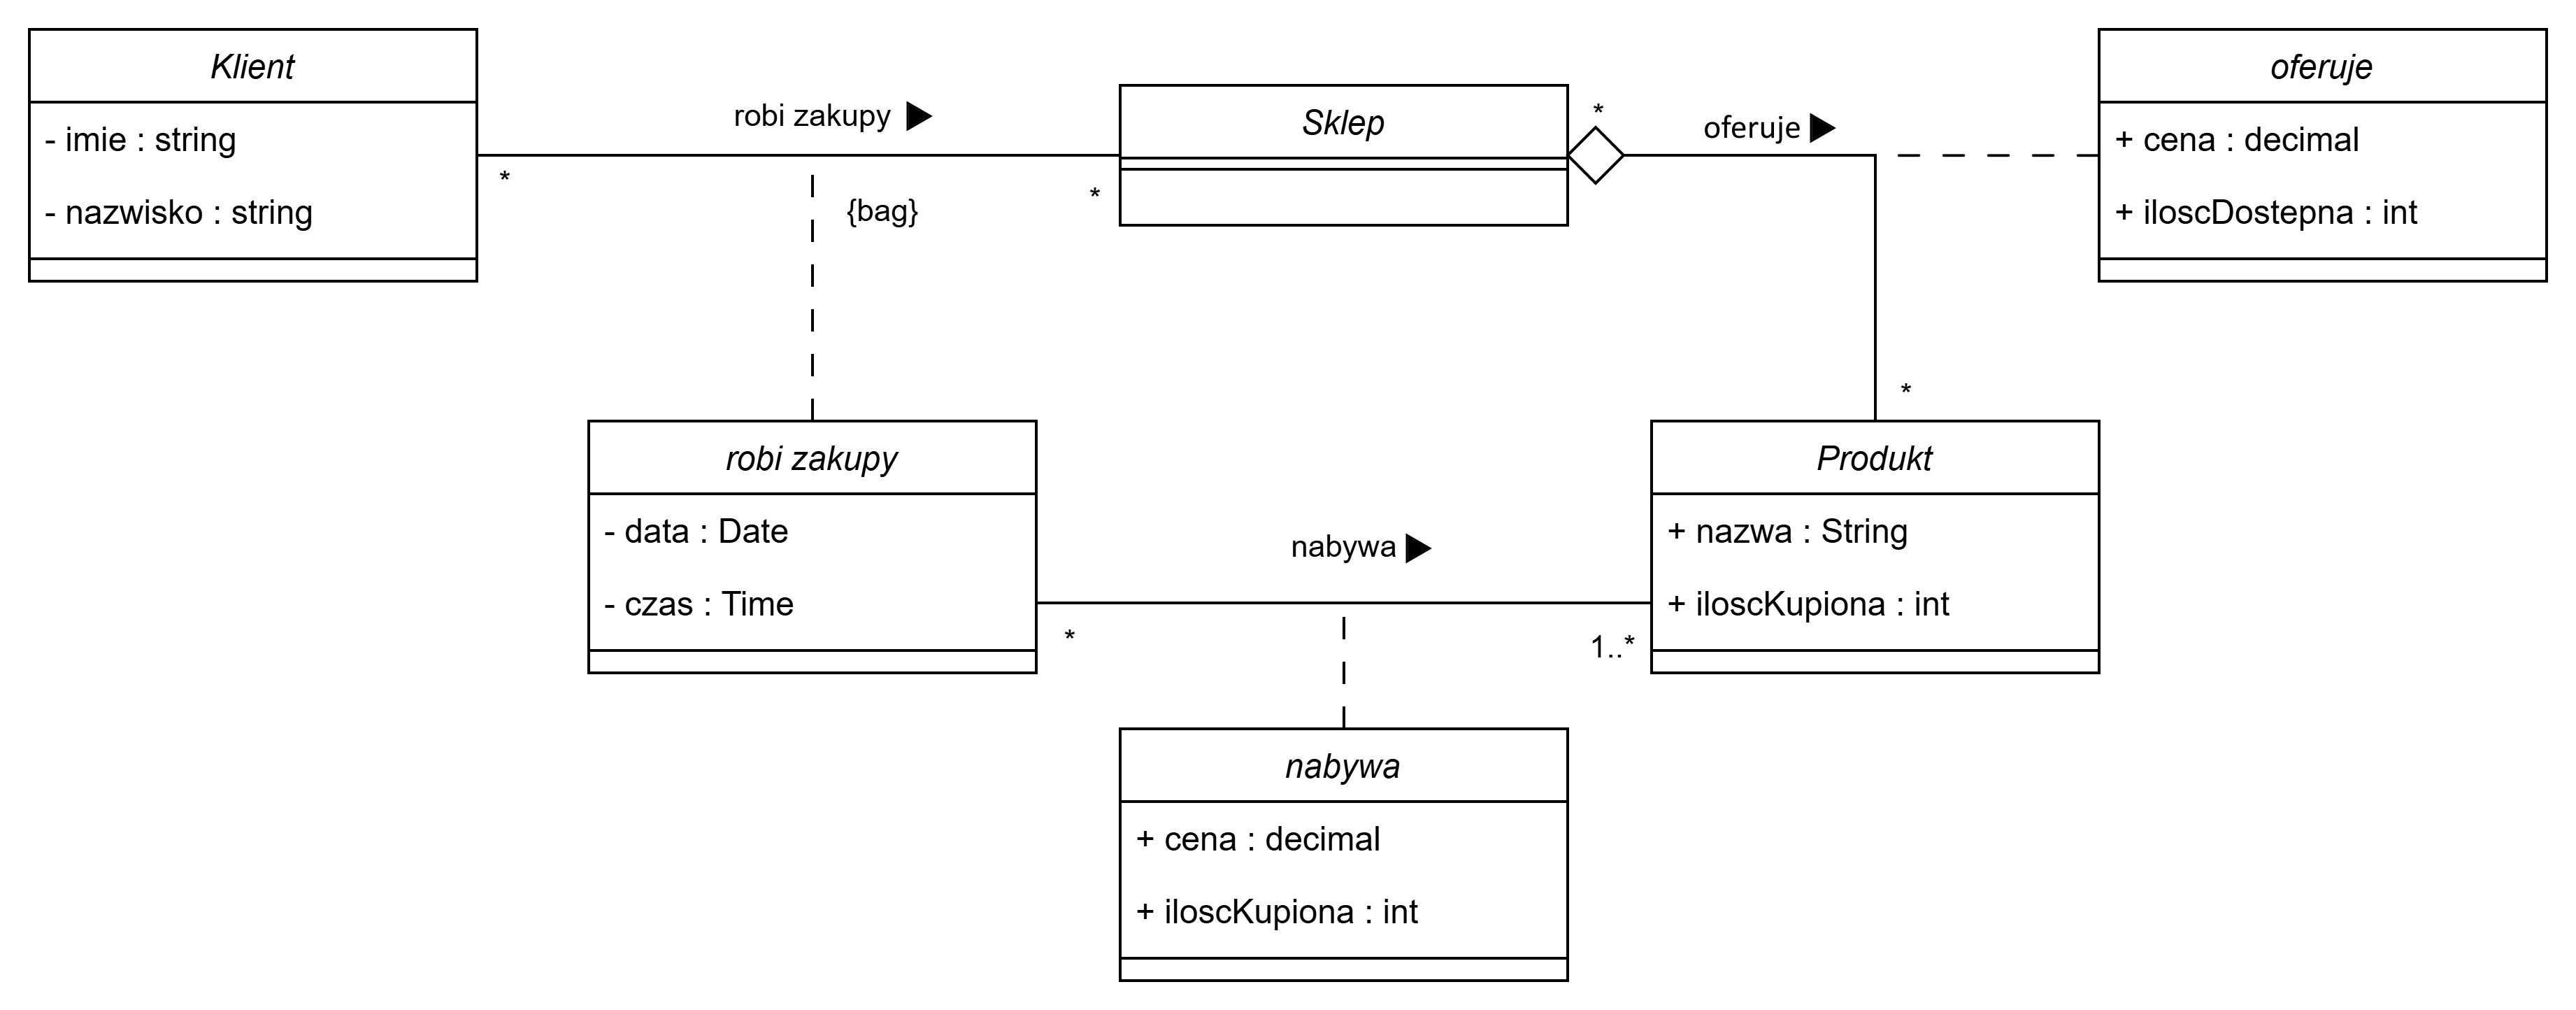
\includegraphics[width=0.8\textwidth]{images/improved.png}
\caption{Finalny model danych "Usługi"}
\label{fig:final_model}
\end{figure}

\subsection{Skrypt DDL SQL}

\begin{lstlisting}[
    language=SQL,
    showspaces=false,
    basicstyle=\ttfamily,
    numbers=left,
    numberstyle=\tiny,
    commentstyle=\color{green}
 ]

 CREATE DATABASE Uslugi;
 GO
 
 USE Uslugi;
 
 DROP TABLE IF EXISTS Nabycie;
 DROP TABLE IF EXISTS Zakup;
 DROP TABLE IF EXISTS Oferta;
 DROP TABLE IF EXISTS Produkt;
 DROP TABLE IF EXISTS Sklep;
 DROP TABLE IF EXISTS Klient;
 
 CREATE TABLE Klient (
     id INT PRIMARY KEY,
     imie VARCHAR(255) NOT NULL,
     nazwisko VARCHAR(255) NOT NULL
 );
 
 CREATE TABLE Sklep (
     id INT PRIMARY KEY,
     nazwa VARCHAR(255) NOT NULL
 );
 
 CREATE TABLE Produkt (
     id INT PRIMARY KEY,
     nazwa VARCHAR(255) NOT NULL UNIQUE
 );
 
 CREATE TABLE Oferta (
     id INT PRIMARY KEY,
     cena DECIMAL(10,2) NOT NULL CHECK (cena >= 0),
     ilosc_dostepna INT NOT NULL CHECK (ilosc_dostepna >= 0),
     sklep_id INT NOT NULL,
     produkt_id INT NOT NULL,
     FOREIGN KEY (sklep_id) REFERENCES Sklep(id) ON DELETE CASCADE,
     FOREIGN KEY (produkt_id) REFERENCES Produkt(id) ON DELETE CASCADE
 );
 
 CREATE TABLE Zakup (
     id INT PRIMARY KEY,
     data DATE NOT NULL,
     czas TIME NOT NULL,
     klient_id INT,
     sklep_id INT NOT NULL,
     FOREIGN KEY (klient_id) REFERENCES Klient(id) ON DELETE SET NULL,
     FOREIGN KEY (sklep_id) REFERENCES Sklep(id) ON DELETE CASCADE,
     CONSTRAINT unique_zakup UNIQUE (data, czas, klient_id, sklep_id)
 );
 
 CREATE TABLE Nabycie (
     id INT PRIMARY KEY,
     cena DECIMAL(10,2) NOT NULL CHECK (cena >= 0),
     ilosc_kupiona INT NOT NULL CHECK (ilosc_kupiona > 0),
     zakup_id INT,
     oferta_id INT,
     FOREIGN KEY (zakup_id) REFERENCES Zakup(id) ON DELETE SET NULL,
     FOREIGN KEY (oferta_id) REFERENCES Oferta(id)
 ); 

\end{lstlisting}

\subsection{Inicjalizacja bazy danych w systemie MS SQL}

\begin{figure}[H]
\centering
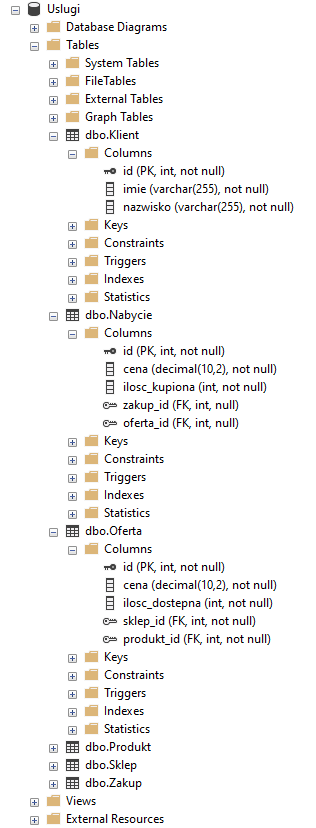
\includegraphics[width=0.8\textwidth]{images/uslugi_db.png}
\caption{Schemat bazy danych "Usługi"}
\label{fig:uslugi_db}
\end{figure}

\subsection{Testy działania bazy danych}

\begin{figure}[H]
    \centering
    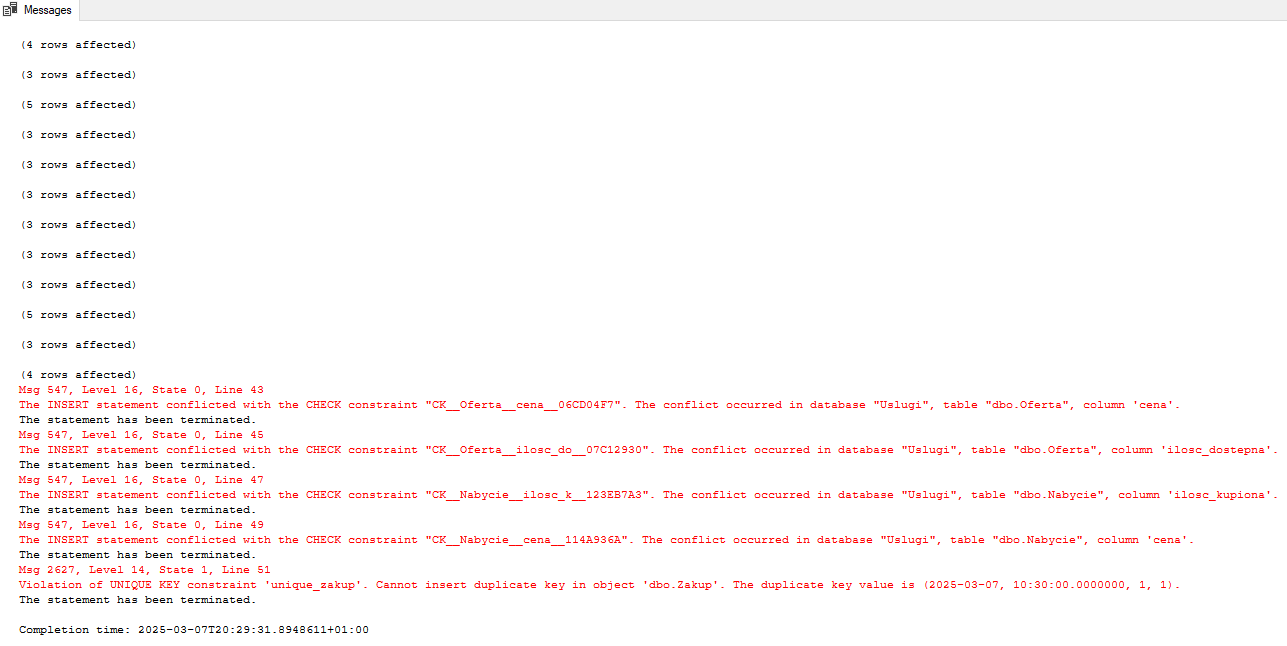
\includegraphics[width=0.8\textwidth]{images/seeding_console.png}
    \caption{Widok konsoli po wykonaniu poniższego kodu}
    \label{fig:tests}
    \end{figure}

\begin{lstlisting}[
    language=SQL,
    showspaces=false,
    basicstyle=\ttfamily,
    numbers=left,
    numberstyle=\tiny,
    commentstyle=\color{green}
    ]

INSERT INTO Klient (id, imie, nazwisko) VALUES
(1, 'Jan', 'Kowalski'),
(2, 'Anna', 'Nowak'),
(3, 'Piotr', 'Wójcik');

INSERT INTO Sklep (id, nazwa) VALUES
(1, 'Biedronka'),
(2, 'Biedronka'),
(3, 'BIEDRONKA pl. GRUNWALDZKI');

INSERT INTO Produkt (id, nazwa) VALUES
(1, 'Masło'),
(2, 'Bułki'),
(3, 'Wędliny');

INSERT INTO Oferta (id, cena, ilosc_dostepna, sklep_id, produkt_id) VALUES
(1, 25.99, 10, 1, 1),
(2, 45.50, 5, 1, 2),
(3, 15.75, 15, 2, 1),
(4, 35.30, 7, 2, 3),
(5, 99.99, 0, 3, 2);

INSERT INTO Zakup (id, data, czas, klient_id, sklep_id) VALUES
(1, '2025-03-07', '10:30:00', 1, 1),
(2, '2025-03-07', '11:00:00', 2, 2),
(3, '2025-03-07', '12:00:00', 3, 3);

INSERT INTO Nabycie (id, cena, ilosc_kupiona, zakup_id, oferta_id) VALUES
(1, 25.99, 3, 1, 1),
(2, 45.50, 2, 2, 2),
(3, 15.75, 5, 3, 3),
(4, 35.30, 1, 3, 4);

-- Invalid operations

INSERT INTO Oferta (id, cena, ilosc_dostepna, sklep_id, produkt_id) VALUES (6, -10.00, 10, 1, 1);

INSERT INTO Oferta (id, cena, ilosc_dostepna, sklep_id, produkt_id) VALUES (7, 20.00, -5, 1, 2);

INSERT INTO Nabycie (id, cena, ilosc_kupiona, zakup_id, oferta_id) VALUES (5, 25.00, 0, 1, 1);

INSERT INTO Nabycie (id, cena, ilosc_kupiona, zakup_id, oferta_id) VALUES (5, -25.00, 1, 1, 1);

INSERT INTO Zakup (id, data, czas, klient_id, sklep_id) VALUES (4, '2025-03-07', '10:30:00', 1, 1);

\end{lstlisting}

Wszystkie operacje zadziałały, oprócz tych, które naruszały ograniczenia. Błędy w konsoli jasno opisują, które konkretnie ograniczenie zostało złamane. Tymi kwerendami sprawdzone zostały wszystkie ograniczenia.

\section{Zadanie 2}

\subsection{Opis zadania}

Do wykonania zadania użyłem bazy danych "AdventureWorks2014" (\url{https://github.com/Microsoft/sql-server-samples/releases/download/adventureworks/AdventureWorks2014.bak})

\begin{figure}[H]
    \centering
    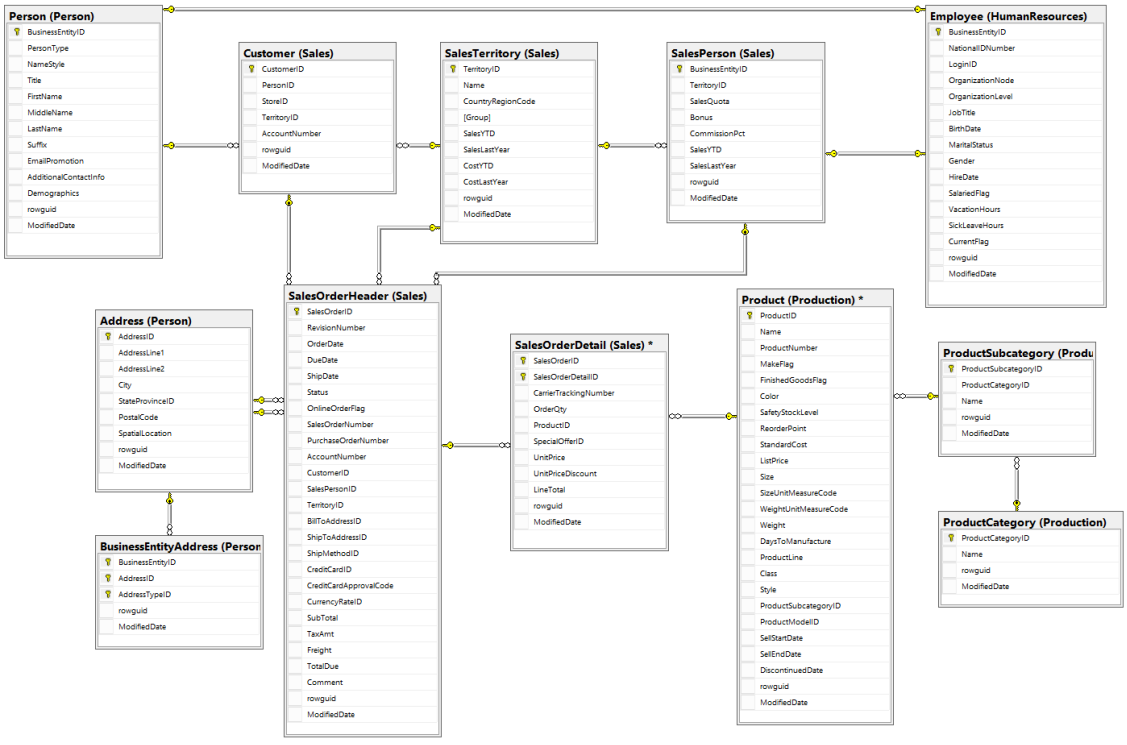
\includegraphics[width=0.8\textwidth]{images/useful_tables.png}
    \caption{Wykorzystane w rozwiązaniu tabele}
    \end{figure}

Kwerendy do wykonania:

\begin{enumerate}
    \item Ile jest produktów w bazie? Ile kategorii i podkategorii?
    \item Wypisz produkty, które nie mają zdefiniowanego koloru.
    \item Podaj roczną kwotę transakcji (SalesOrderHeader.TotalDue) w poszczególnych latach.
    \item Ilu jest klientów, a ilu sprzedawców w sklepie? Ilu w poszczególnych regionach?
    \item Ile było wykonanych transakcji w poszczególnych latach?
    \item Podaj produkty, które nie zostały kupione przez żadnego klienta. Zestawienie pogrupuj według kategorii i podkategorii.
    \item Oblicz minimalną i maksymalną kwotę rabatu udzielonego na produkty w poszczególnych podkategoriach.
    \item Podaj produkty, których cena jest wyższa od średniej ceny produktów w sklepie.
    \item Ile średnio produktów w każdej kategorii sprzedaje się w poszczególnych miesiącach?
    \item Ile średnio czasu klient czeka na dostawę zamówionych produktów? Przygotuj zestawienie w zależności od kodu regionu (SalesTerritory.CountryRegionCode).
\end{enumerate}

\subsection{Kwerendy}

\begin{figure}[H]
    \centering
    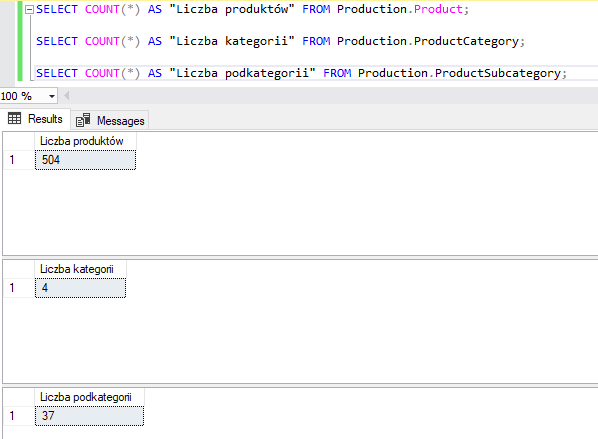
\includegraphics[width=0.8\textwidth]{images/01.png}
    \caption{Wynik kwerendy 1}
    \end{figure}

\begin{figure}[H]
    \centering
    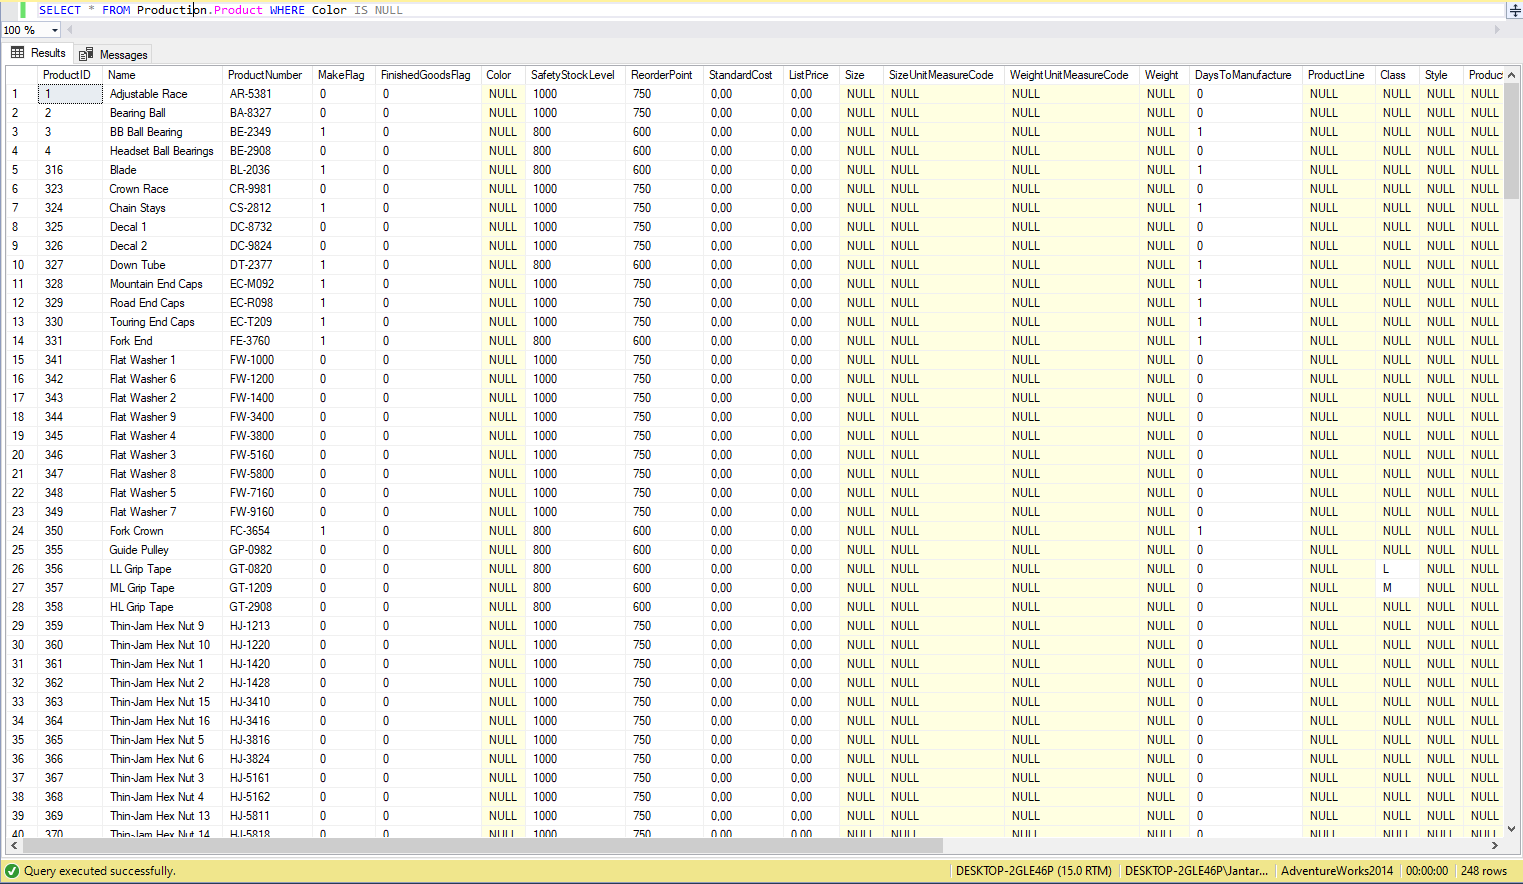
\includegraphics[width=0.8\textwidth]{images/02.png}
    \caption{Wynik kwerendy 2}
    \end{figure}

\begin{figure}[H]
    \centering
    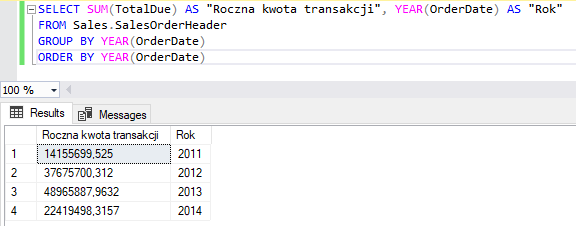
\includegraphics[width=0.8\textwidth]{images/03.png}
    \caption{Wynik kwerendy 3}
    \end{figure}

\begin{figure}[H]
    \centering
    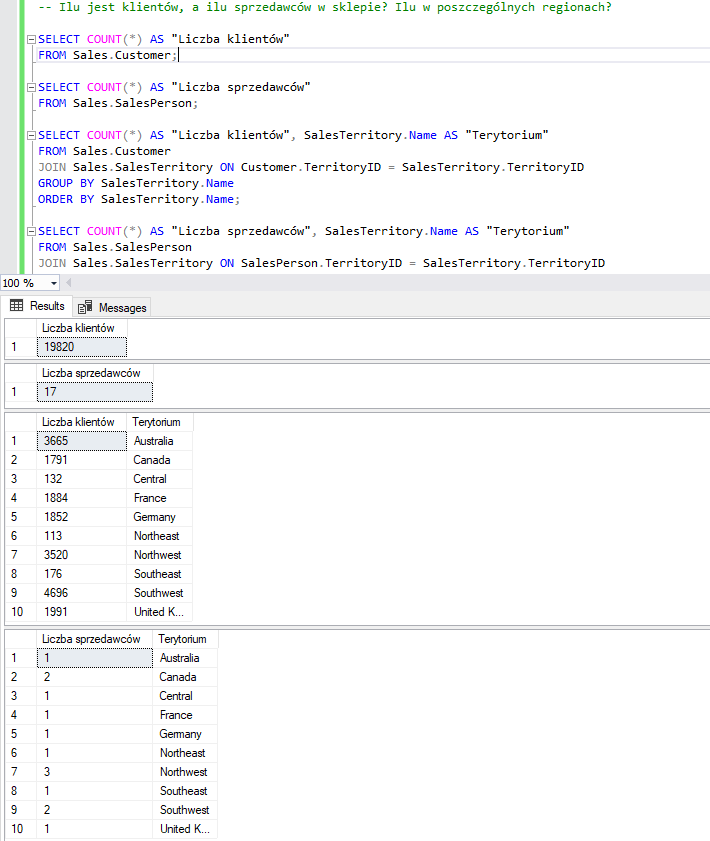
\includegraphics[width=0.8\textwidth]{images/04.png}
    \caption{Wynik kwerendy 4}
    \end{figure}

\begin{figure}[H]
    \centering
    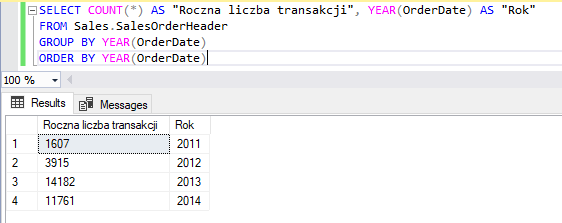
\includegraphics[width=0.8\textwidth]{images/05.png}
    \caption{Wynik kwerendy 5}
    \end{figure}

\begin{figure}[H]
    \centering
    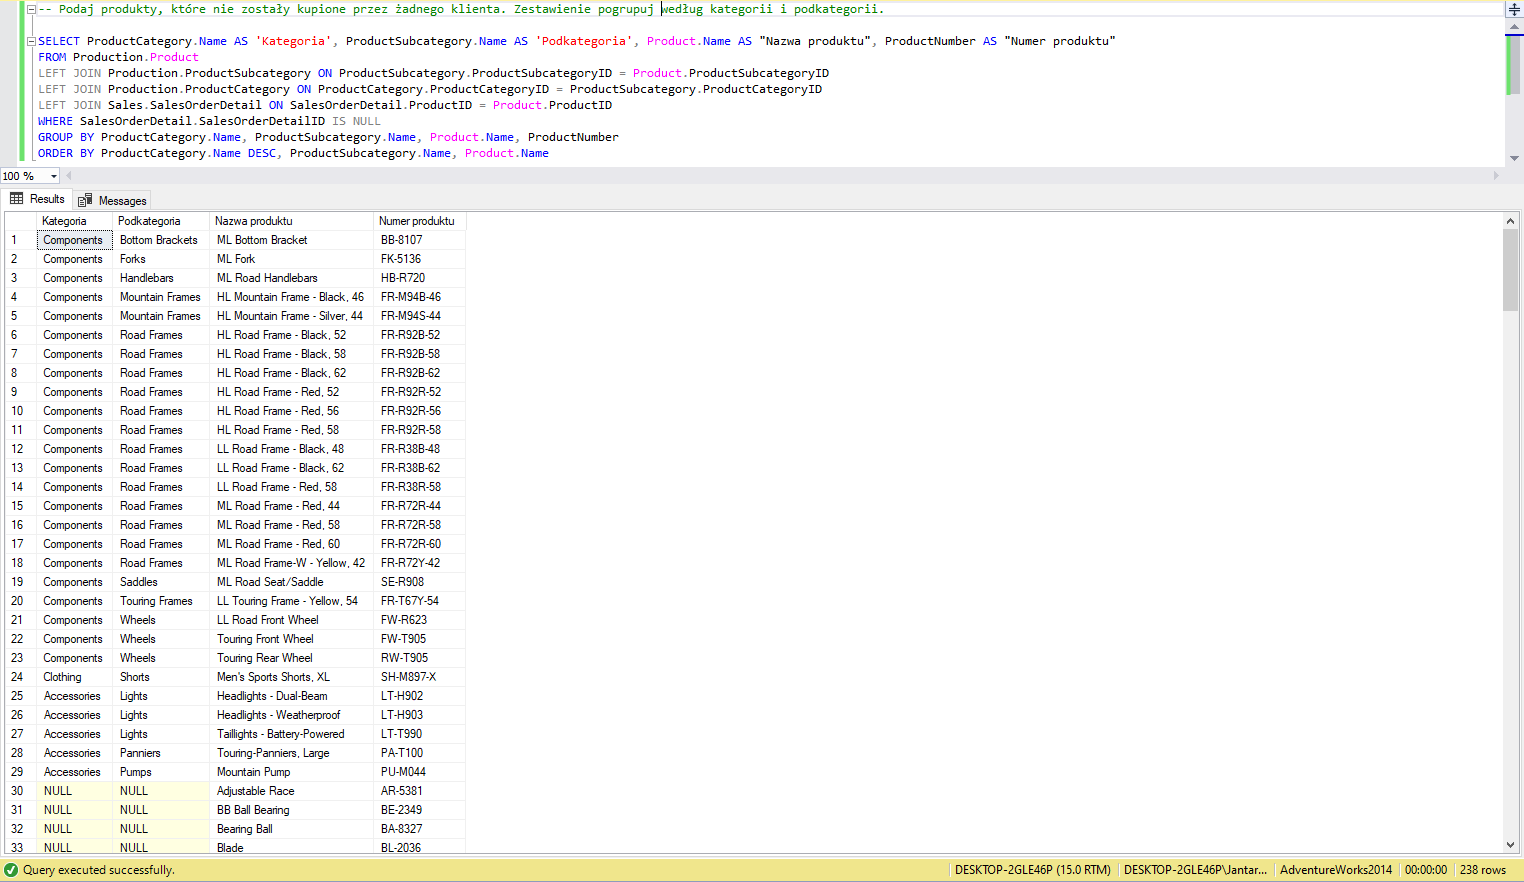
\includegraphics[width=0.8\textwidth]{images/06.png}
    \caption{Wynik kwerendy 6}
    \end{figure}

\begin{figure}[H]
    \centering
    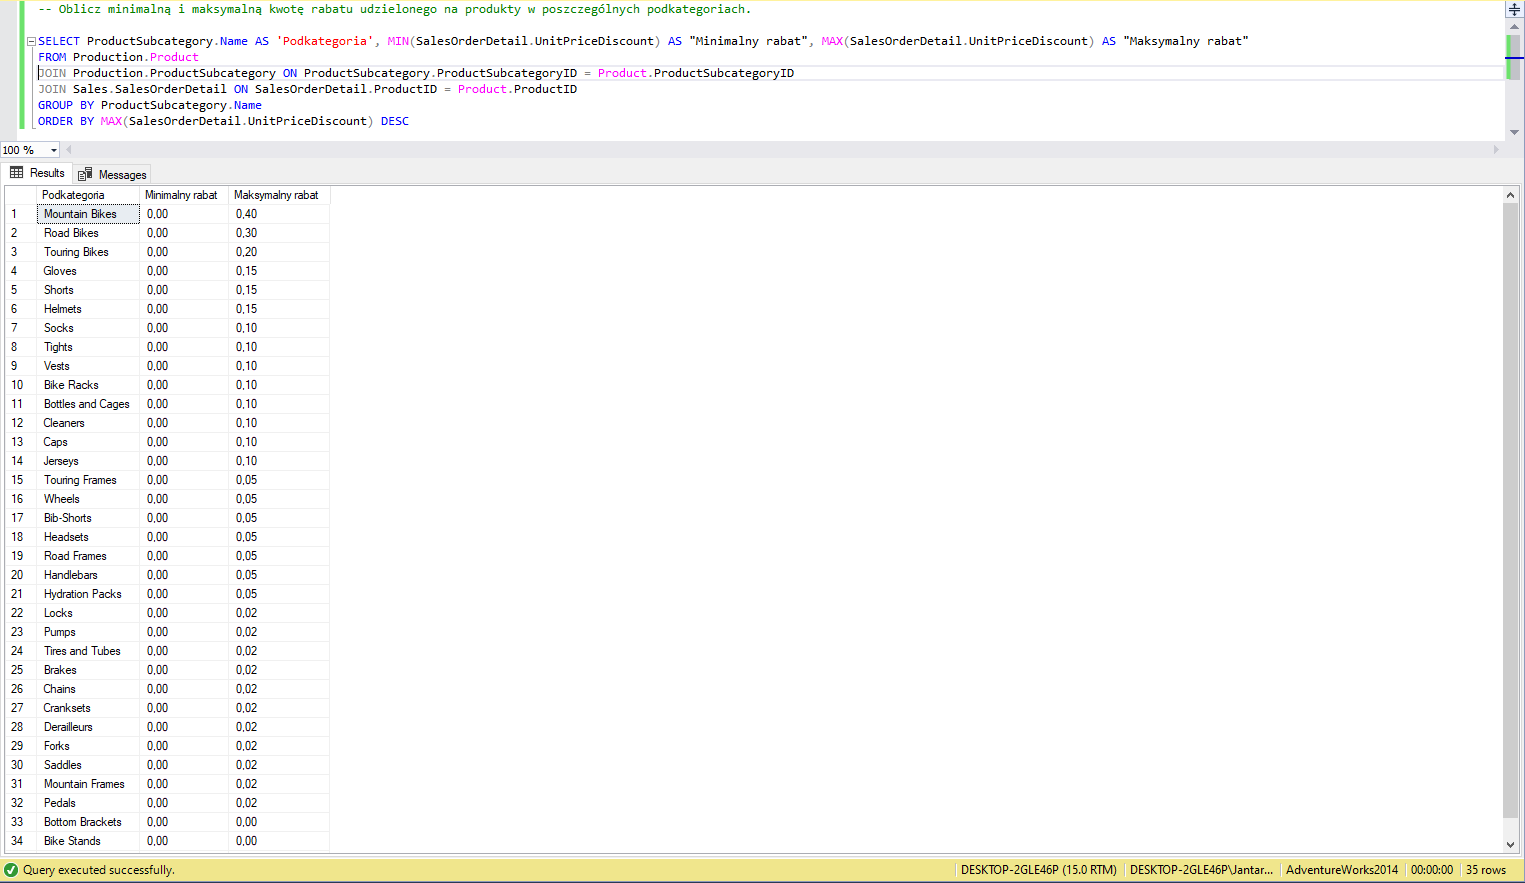
\includegraphics[width=0.8\textwidth]{images/07.png}
    \caption{Wynik kwerendy 7}
    \end{figure}

\begin{figure}[H]
    \centering
    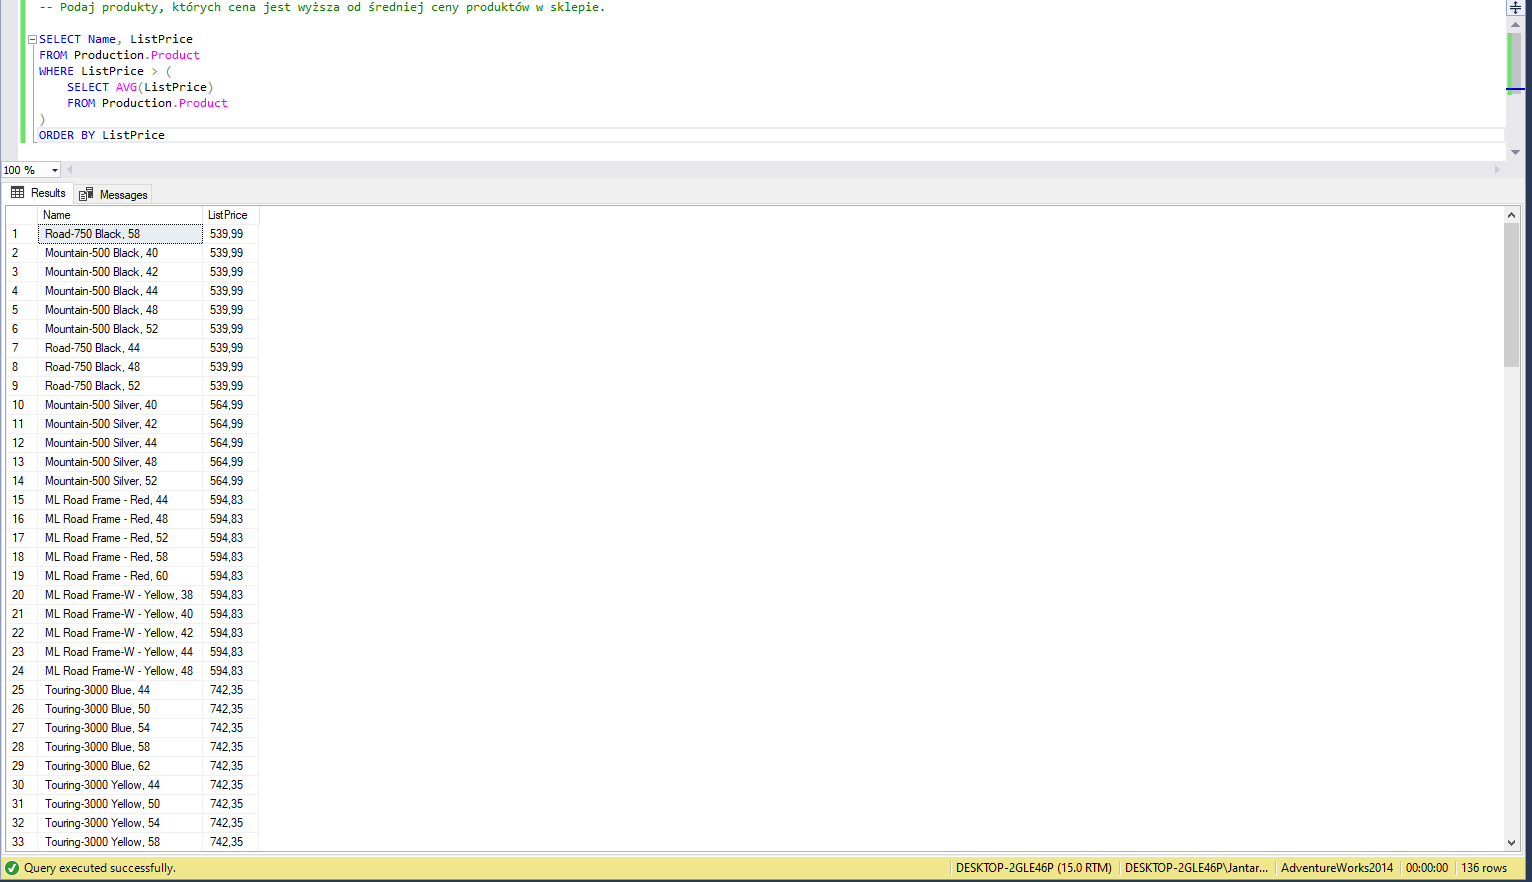
\includegraphics[width=0.8\textwidth]{images/08.png}
    \caption{Wynik kwerendy 8}
    \end{figure}

\begin{figure}[H]
    \centering
    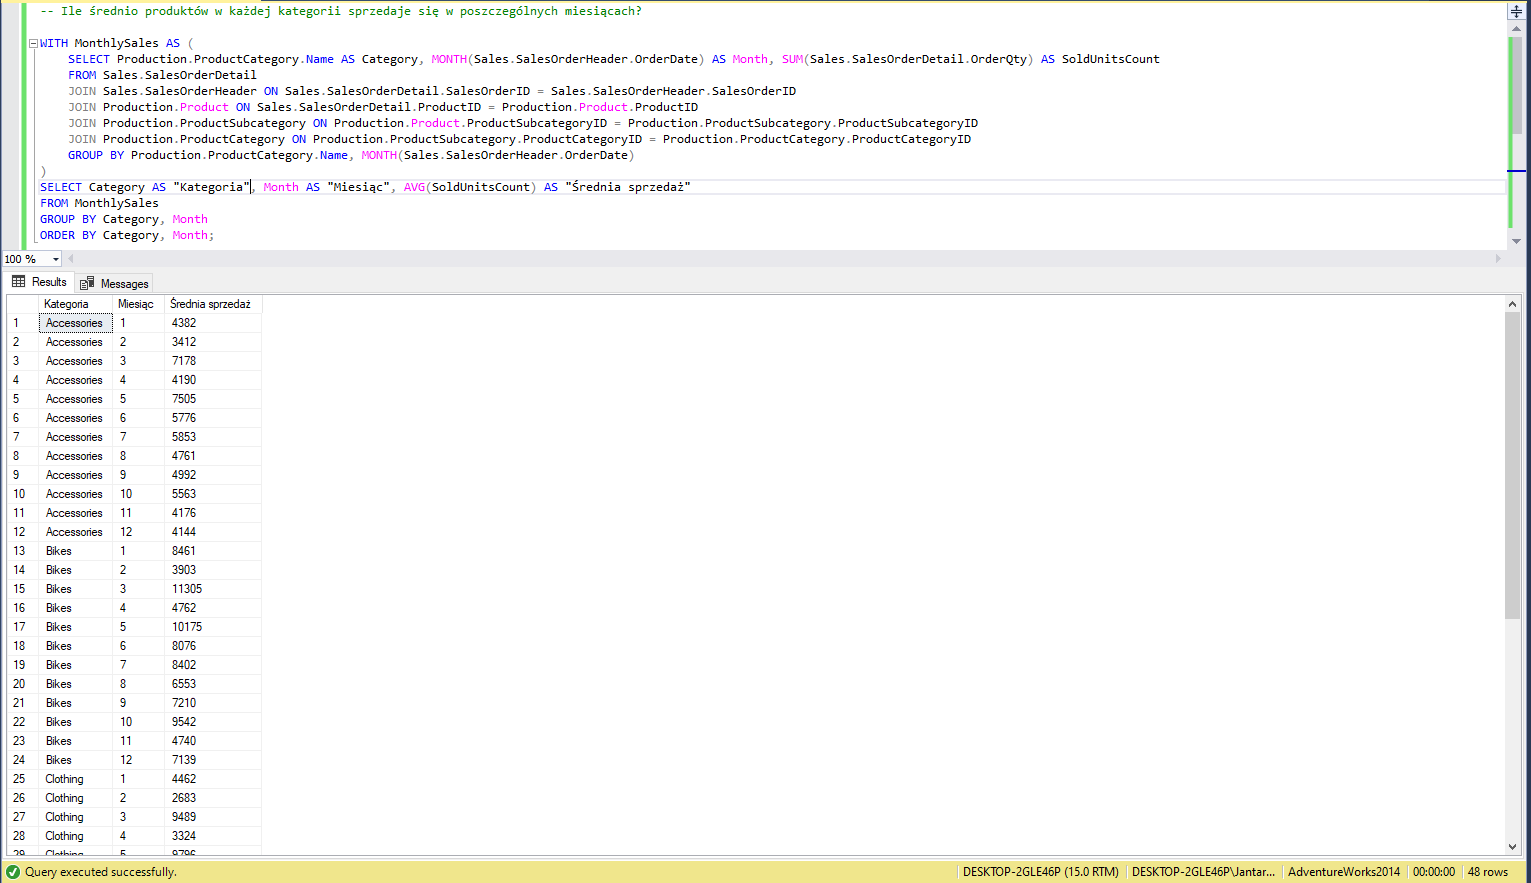
\includegraphics[width=0.8\textwidth]{images/09.png}
    \caption{Wynik kwerendy 9}
    \end{figure}

\begin{figure}[H]
    \centering
    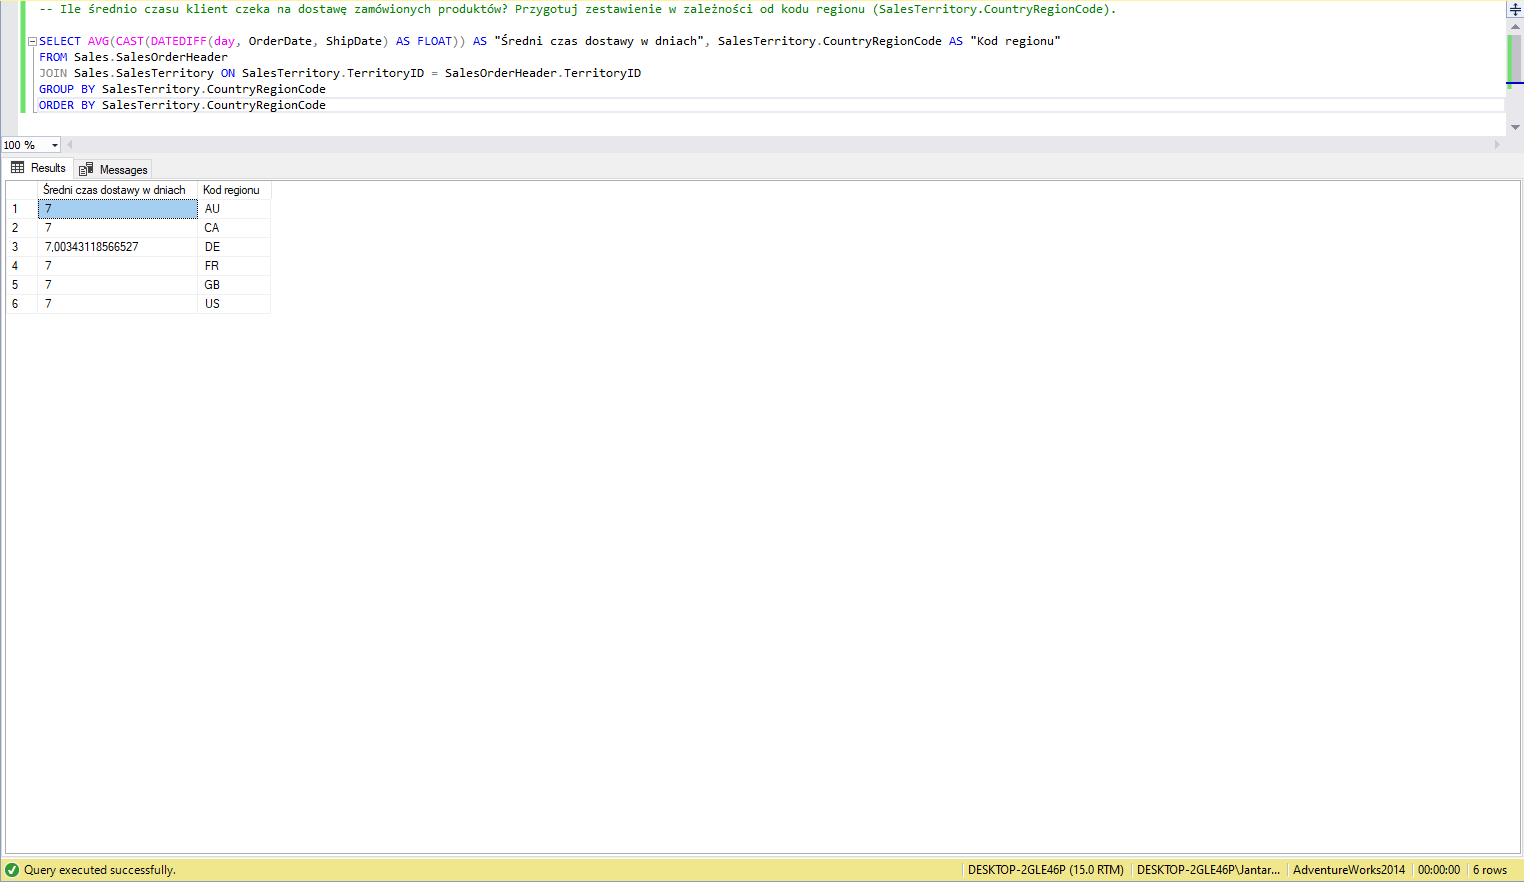
\includegraphics[width=0.8\textwidth]{images/10.png}
    \caption{Wynik kwerendy 10}
    \end{figure}

\section{Wnioski}

\subsection{Wnioski z zadania 1}

Zadanie okazało się znacznie bardziej skomplikowane, niż mogło by się wydawać na pierwszy rzut oka. Im więcej czasu spędzi się nad takim z pozoru prostym diagramem, tym więcej można dodać reguł do uściślenia zasad. Bez jasnych wytycznych klienta można też było przyjąć zupełnie inne założenia wobec bazy danych. Aktualna wersja bazy danych jest dość abstrakcyjna - nie jest jasne, czy dotyczy tylko sklepów internetowych, czy stacjonarnych, czy obu naraz. Moim zamysłem było nie ograniczać za bardzo możliwości, tak więc aktualną tabelę można by wykorzystać do obu rodzajów sklepów.

W przykładowych danych, którymi zasiałem bazę, widać już pewne usprawnienie - prawdopodobnie w przyszłości można by wyciągnąć kategorię sklepu do osobnej tabeli, aby, na przykład, mieć pewność, że wszystkie sklepy konkretnej marki będą łatwo dostępne. Wtedy każdy z tych sklepów byłby np. kategorii "Biedronka". Można by przekształcić też kategorię w kierunku opisu innych właściwości sklepu, np. czy jest internetowy, czy stacjonarny.

Podsumowując, liczba reguł znacznie wzrosła, ale bez jasnych wytycznych klienta warto ograniczyć się w ich ilości, żeby zezwalać na więcej możliwości w przyszłości. Oczywiście, jedyną pewną rzeczą w oprogramowaniu jest ciągła zmiana, ale nowoczesne narzędzia bazodanowe są w stanie bardzo wspomóc migracje do nowych wytycznych.
Tak więc nie trzeba przesadnie "bać" się różnych pomysłów w początkowej fazie projektowania, byleby je dobrze i ciągle konsultować z klientem.

\subsection{Wnioski z zadania 2}

Pewne jest to, że te 10 kwerend to było zdecydowanie za mało, by dowiedzieć się wszystkiego o stanie omawianej firmy. To też za mało, żeby próbować zrozumieć czynniki wpływające na taką, a nie inną, sytuację. Ale mimo tego, można i tak wywnioskować ciekawe informacje.

Oferta sklepu wydaje się dość różnorodna i logicznie podzielona na kategorie i podkategorie. Sklep z każdym rokiem wydaje się zarabiać coraz więcej (mogłoby się wydawać, że w roku 2014 jest spadek, ale zapisy w bazie danych kończą się w połowie roku). 

Liczba klientów jest dość spora, zwłaszcza, jak na liczbę sprzedawców. Korelacja między liczbą klientów a liczbą sprzedawców w danym regionie wydaje się istnieć (więcej klientów -> więcej sprzedawców). Wyjątkiem jest Kanada - w innych regionach jest tylko 1 sprzedawca dla tylu klientów. Rozkład klientów na pewno nie jest równomiernie podzielony na regiony - region Southeast i Northeast wydają się radzić sobie z nimi najgorzej (być może z dalszych badań udałoby się odkryć przyczynę).

Liczba transakcji zdecydowanie wzrasta z każdym rokiem. Zarobki wzrastają jednak wolniej, co oznacza, że średnia wartość transakcji spadła w późniejszych latach.

Aż połowa produktów nigdy nie została sprzedana. Być może oferta jest zbyt różnorodna, być może zostały wprowadzone bardzo niedawno - bez dalszych badań nie wiadomo.

Sklep nie zawsze udziela rabatów. Maksymalne wartości rabatów wydają się umiarkowane. Przydałoby się poznać średnią wartość rabatu, bo maksimum i minimum daje nam za mało informacji.

Próg średniej ceny przekracza ponad 1/4 produktów. Wydaje się to być standardową sytuacją.

Zauważalny jest wzrost sprzedaży w miesiącach letnich, co było do przewidzenia dla sklepu rowerowego.

Średni czas oczekiwania klienta w zależności od regionu jest podejrzany. W aż 5 z 6 regionów średni czas wynosi dokładnie 7 dni.

Podsumowując, udało się odkryć część informacji dotyczących sklepu. Bez dalszych badań można jedynie przypuszczać, co mogło być powodem takich, a nie innych, wyników.

\end{document}